\documentclass{article}
\usepackage{graphicx}
\usepackage{polski}
\usepackage{listings}

\renewcommand{\figurename}{Wykres}
\renewcommand{\lstlistingname}{Kod}

\title{Mnożenie macierzy}
\author{Szymon Twardosz, Dominik Jeżów}
\date{\today}

\begin{document}

\maketitle

\section{\'Srodowisko}
Do wykonania \'cwiczenia wykorzystali\'smy język
python 3.11 wraz z nast\k{e}puj\k{e}cymi bibliotekami
numpy, matplotlib oraz time

\section{Temat zadania}
Zadanie polegało na zaimplementowaniu 3 różnych metod mnożenia macierzy kwadratowych o wymiarach
będących potęgą liczby 2. Są to kolejno:
\begin{description}
\item[Metoda Binet'a] Najprostsza metoda rekurencyjna polegająca na obliczeniu
macierzy wynikowej na podstawie 4 oddzielnych fragmentów
\item[Metoda Strassena] Podobna do powyższej metody z tą różnicą, że dzielimy
macierz na więcej części, aby zmniejszyć ilość wykonanych operacji arytmetycznych.
\item[Metoda Alpha Tensor] Tak jak wyżej tylko, że ilość, na którą została
podzielona macierz, jest znaleziona przez model sztucznej inteligencji.
(Przy tej metodzie nie korzystaliśmy z powyższej zasady co do wielkości macierzy,
a za to mnożyliśmy macierze ($4^n$, $5^n$) $\times$ ($5^n$, $5^n$))
\end{description}

\section{Opis fragmentów kodu}
\subsection{Metoda Binet'a}
\begin{lstlisting}
  def binet(A: np.ndarray, B: np.ndarray):
    ...

    A11, A12, A21, A22 = divide_matrix(A, n)
    B11, B12, B21, B22 = divide_matrix(B, n)

    C11 = binet(A11, B11) + binet(A12, B21)
    C12 = binet(A11, B12) + binet(A12, B22)
    C21 = binet(A21, B11) + binet(A22, B21)
    C22 = binet(A21, B12) + binet(A22, B22)

    # Add number of adding to flops

    return np.vstack(
        (np.hstack((C11, C12)),
         np.hstack((C21, C22)))
    )
    
\end{lstlisting}
\subsection{Mestoda Strassena}

\begin{lstlisting}
  def strassen(A, B):
    ...

    A11, A12, A21, A22 = divide_matrix(A, n)
    B11, B12, B21, B22 = divide_matrix(B, n)

    P1 = strassen(A11 + A22, B11 + B22)
    P2 = strassen(A21 + A22, B11)
    P3 = strassen(A11, (B12 - B22))
    P4 = strassen(A22, (B21 - B11))
    P5 = strassen(A11 + A12, B22)
    P6 = strassen(A21 - A11, B11 + B12)
    P7 = strassen(A12 - A22, B21 + B22)


    return np.vstack(
        (np.hstack((P1 + P4 - P5 + P7, P3 + P5)),
        np.hstack((P2 + P4, P1 - P2 + P3 + P6)))
    )

\end{lstlisting}
\subsection{Metoda Alpha Tensor}
\begin{lstlisting}
  def alpha_tensor(A: np.ndarray, B: np.ndarray):
    ...

    # Calculating matrix C
    C11 = -h[10] + h[12] + h[14] - h[15] - h[16] + h[53] + h[5] - h[66] - h[7]
    C21 = h[10] + h[11] - h[12] + h[13] + h[15] + h[16] - h[17] - h[44] + h[51]
    C31 = h[10] - h[12] + h[15] + h[16] - h[1] + h[2] + h[3] - h[4] + h[75]
    C41 = -h[10] + h[12] - h[15] - h[16] + h[52] + h[54] - h[6] - h[8] + h[9]
    C12 = h[13] + h[15] + h[20] + h[21] - h[22] + h[23] + h[25] - h[43] + h[49] + h[50]
    C22 = -h[11] + h[12] - h[13] - h[15] - h[16] + h[17] + h[18] - h[19] - h[21] + h[43] + h[44]
    C32 = -h[16] - h[19] - h[21] - h[28] - h[29] - h[38] + h[42] + h[44] - h[47] + h[48]
    C42 = h[11] - h[12] - h[18] + h[21] - h[32] + h[33] - h[34] - h[36] + h[62] - h[70]
    C13 = h[15] + h[23] + h[24] + h[34] - h[37] + h[40] - h[41] + h[55] - h[56] - h[9]
    C23 = -h[10] + h[19] + h[32] + h[35] + h[36] + h[37] - h[43] - h[60] - h[6] - h[72]
    C33 = -h[16] - h[28] + h[33] + h[37] - h[39] + h[45] - h[46] + h[63] - h[71] - h[8]
    C43 = h[10] + h[15] + h[16] - h[33] + h[34] - h[35] - h[37] - h[54] + h[6] + h[8] - h[9]
    C14 = -h[10] + h[12] + h[14] - h[16] + h[23] + h[24] + h[25] + h[26] + h[5] - h[66] - h[7]
    C24 = h[10] + h[18] - h[19] + h[20] - h[22] - h[24] - h[26] - h[5] - h[69] + h[73]
    C34 = -h[14] + h[16] - h[23] - h[26] + h[27] + h[29] + h[31] + h[46] - h[58] + h[76]
    C44 = h[12] + h[25] + h[26] - h[33] - h[35] - h[40] + h[41] + h[65] - h[68] - h[7]
    C15 = h[15] + h[24] + h[25] + h[27] - h[28] + h[30] + h[31] - h[4] + h[61] + h[64]
    C25 = -h[10] - h[18] - h[2] - h[30] - h[38] + h[42] - h[43] + h[46] + h[67] + h[74]
    C35 = -h[10] + h[12] - h[15] + h[28] + h[29] - h[2] - h[30] - h[3] + h[46] + h[4] - h[75]
    C45 = -h[12] - h[29] + h[30] - h[34] + h[35] + h[39] + h[3] - h[45] + h[57] + h[59]

    return np.vstack(
        (np.hstack((C11, C12, C13, C14, C15)),
         np.hstack((C21, C22, C23, C24, C25)),
         np.hstack((C31, C32, C33, C34, C35)),
         np.hstack((C41, C42, C43, C44, C45)),)
    )
\end{lstlisting}
\paragraph*{Opis kodów:}
Jak widać Powyrzsze znacznie się nie różnią, a składają się z trzech kroków:
\begin{itemize}
  \item przygotowanie podzielonych macierzy
  \item obliczenie kawałków (C\_i) macierzy Wynikowej C
  \item złożenie macierzy C
\end{itemize}
Jedyne co się zmieia to ilość podziałów macierzy. Dodatkowo w metodzie Alpha Tensor liczba wyliczanych kawałków to 20 a nie jak w innych metodach - 4
\section{Przykład}
Jak widać na podsawie poniższego przykładu nasza implementacja metod dzała poprawnie
\begin{lstlisting}[language=Matlab, caption=Kod MATLAB]
  A = [1, 2; 3, 4];  
  B = [5, 6; 7, 8];
  C = A * B;  
  disp(C)

  % 19   22
  % 43   50
  %  45    60    75    90    45
  % 110   140   170   200    70
  %  45    60    75    90    45
  % 110   140   170   200    70
  \end{lstlisting}
  \begin{lstlisting}[language=Python, caption=Wynik]
    A = np.array([[1, 2],[ 3, 4]])
    B = np.array([[5, 6],[ 7, 8]])
    
    A2 = np.array(
        [
            [1, 2, 3, 4, 5],
            [6, 7, 8, 9, 0],
            [1, 2, 3, 4, 5],
            [6, 7, 8, 9, 0]
        ]
    )
    B2 = np.array(
        [
            [1, 2, 3, 4, 5],
            [6, 7, 8, 9, 0],
            [1, 2, 3, 4, 5],
            [6, 7, 8, 9, 0],
            [1, 2, 3, 4, 5]
        ]
    )
    
    print(binet(A, B))
    print(strassen(A, B))
    print(alpha_tensor(A2, B2))

%   [[19 22]
%   [43 50]]
%   [[19 22]
%   [43 50]]
%   [[ 45.  60.  75.  90.  45.]
%   [110. 140. 170. 200.  70.]
%   [ 45.  60.  75.  90.  45.]
%   [110. 140. 170. 200.  70.]]
    \end{lstlisting}

\section{Wyniki}
\subsection*{Czasy obliczeń}

\begin{description}
\item[Metoda Binet'a]  Dla największych macierzy, jakie zbadaliśmy czas liczenia wynosił około 20 minut.
\item[Metoda Strassena]Metoda ta otrzymała wyniki w najszybszym czasie — dla macierzy kwadratowych
o wymiarze 516 otrzymał wynik w czasie ponad 2 razy szybszym od metody Binet'a.
\item[Metoda Alpha Tensor] Posiadał najgorsze wyniki czasowe, dla macierzy z liczbą elementów
większą od 200 obliczenia trwały dłużej niż 30 minut (nie wyliczaliśmy
ich do końca). Trzeba zwrócić uwagę na to, że funkcje tworzą macierze o rozmiarach ($4^n$, $5^n$)
co przyczyniło się do większej ilości czasu potrzebnego na obliczenia, oraz małej ilości danych do analizowania.
\end{description}

\subsection*{flopsy}

\begin{description}
\item[Metoda Binet'a] Metoda ta miała największą ilość działań arytmetycznych
\item[Metoda Strassena] Metoda wykonuje znacznie mniej działań arytmetycznych
\item[Metoda Alpha Tensor] Metoda ta radzi sobie podobnie do metody Strassena, choć trudno powiedzieć co się dzieje dalej, gdyż czasy wykonania na to nie pozwalały.
\end{description}

\section{Wnioski}
\begin{itemize}
  \item Mestoda Strassena najlepiej poradziła sobie z macierzami.
  \item Metoda Alpha Tensor pomimo że miała mniej więcej tyle samo flops'ów co metoda Strassena poradziła sobie najgożej ze wszystkich metod.
  \item W niewielkim koszcie implementacyjnym otrzymaliśmy leprze czasy od rekurencyjnej metody Binet'a
\end{itemize}
\section*{}
\begin{figure}
\centering
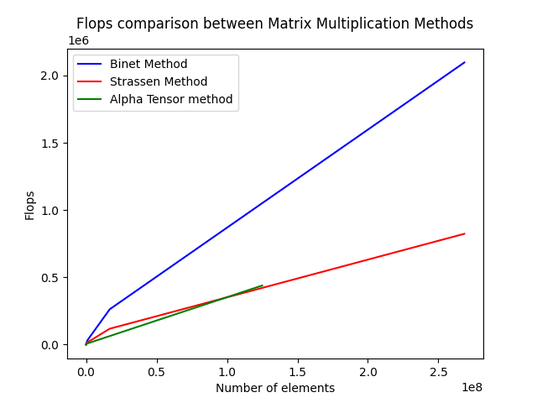
\includegraphics[width=0.8\textwidth]{output.png}
\caption{Porównanie wykonanych operacji arytmetycznych}
\end{figure}
\begin{figure}
\centering
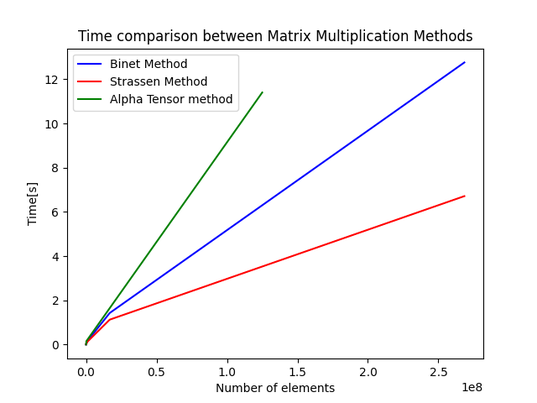
\includegraphics[width=0.8\textwidth]{output2.png}
\caption{Porównanie czasów wykonania}
\end{figure}
\end{document}